\documentclass[11pt,a4paper]{article}

\usepackage{graphicx}
\usepackage{url}
\title{Enabling I2C interface in Raspberry Pi.}
\author{e-Yantra Team}
\date{\today}

\begin{document}
	\maketitle
	\newpage
	\tableofcontents
	\newpage
	\section{Objective}
	In this tutorial we will learn how to enable I2C Interface in Raspberry Pi.
	\section{Prerequisites}
	One should have:
	\begin{itemize}
		\item To know to do interconnections on bread board.
		\item Knowledge of how to do SSH connection.
		\item Some basic information regarding different serial communication \newline protocols
	\end{itemize}
	\section{Hardware Requirement}
	\begin{enumerate}
		\item Raspberry Pi (I will be using Version 2 Model B+)
		\item Power adapter
		\item Connecting wires
		\item Bread board
	\end{enumerate}
	\section{Software Requirement}
	MobaXterm (for windows user) 
	
	\newpage
	\section{Theory and Description}
	The no. of GPIO pins in an R-Pi is less(merely 26 in R-Pi 2) and so interfacing sensors and other modules would consume most of the pins thus setting a limit for I/O access. Therefore in order to increase the no. of GPIO pins we can interface a port expander to an R-Pi.
	
	A port expander is a hardware device designed to allow a user to utilize more than one device on a single port at one time. For example, the device may allow seven devices to connect to one serial port.[1]
	
	\subsection{I2C}
	I2C (Inter-Integrated Circuit), pronounced I-squared-C, is a multi-master, multi-slave, single-ended, serial computer bus used for attaching lower-speed peripheral ICs to processors and micro controllers.[2]
	
	The two I2C signals are called 'serial data’ (SDA) and ‘serial clock’ (SCL). There is no need of chip select (slave select) or arbitration logic in this. Virtually any number of slaves and any number of masters can be connected onto these 2 signal lines and communicate between each other using a protocol that defines:
	\begin{itemize}
			\item 7-bits slave addresses: each device connected to the bus has got such a unique address
			\item data divided into 8-bit bytes
			\item a few control bits for controlling the communication start, end, direction and for an acknowledgement mechanism.
	\end{itemize}

	The data rate has to be chosen between 100 kbps, 400 kbps and 3.4 Mbps, respectively called standard mode, fast mode and high speed mode. Some I²C variants include 10 kbps (low speed mode) and 1 Mbps (fast mode +) as valid speeds.
	
	Physically, the I2C bus consists of the 2 active wires SDA and SCL and a ground connection. The active wires are both bi-directional.[3] 
	\begin{figure}[h!]
		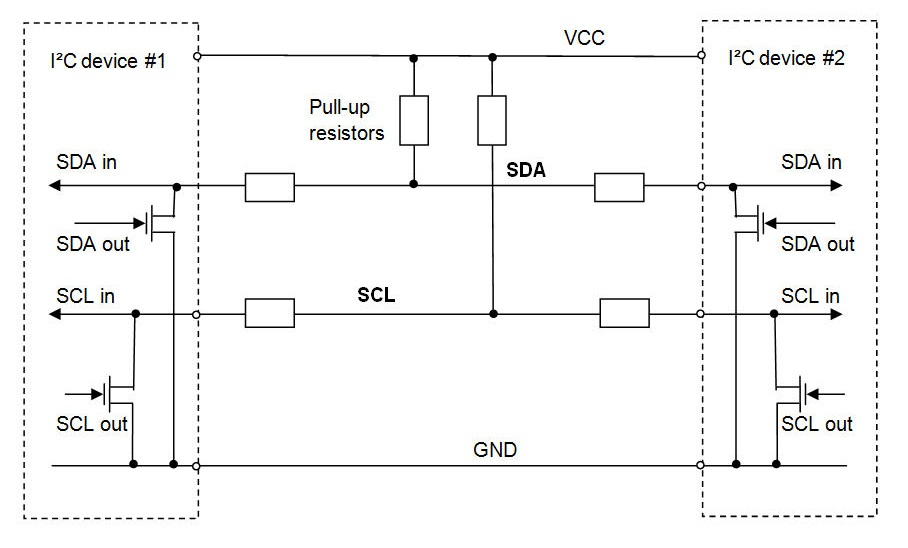
\includegraphics[scale=0.4]{i2c.jpg}
		\centering
		\caption{[3]}
	\end{figure} 
	
	\newpage
	The I2C protocol specification states that the IC that initiates a data transfer on the bus is considered the Bus Master. Consequently, at that time, all the other ICs are regarded to be Bus Slaves. 
	
	\flushleft
	\textbf{Data transfer using I2C}
	\begin{enumerate}
		\item First, the master will issue a START condition. This acts as an ‘Attention’ signal to all of the connected devices. All ICs on the bus will listen to the bus for incoming data.
		\item Then the master sends the ADDRESS of the device it wants to access, along with an indication whether the access is a Read or Write operation. Having received the address, all IC’s will compare it with their own address. If it doesn’t match, they simply wait until the bus is released by the stop condition. If the address matches, however, the chip will produce a response called the ACKNOWLEDGE signal.
		\item Once the master receives the acknowledgement, it can start transmitting or receiving DATA.When all is done, the master will issue the STOP condition. This is a signal that states the bus has been released and that the connected ICs may expect another transmission to start any moment.
		\item When a master wants to receive data from a slave, it proceeds the same way, but sets the R/W bit at a logical one. Once the slave has acknowledged the address, it starts sending the requested data, byte by byte. After each data byte, it is up to the master to acknowledge the received data.[3]
	\end{enumerate}
	
	\subsection{Enabling I2C interface on R-Pi}
	\begin{enumerate}
		\item Open MobaXterm. 
		\item Establish SSH connection to R-Pi.
		\item Under Advanced SSH settings.
		\subitem If in remote environment you have chosen Interactive shell.
		\subitem If in remote environment you have chosen LXDE desktop then open LXTerminal.
		
		\item  Type \textit{sudo raspi-config}. This will launch the raspi-config utility.
		
		\begin{figure}[h!]
			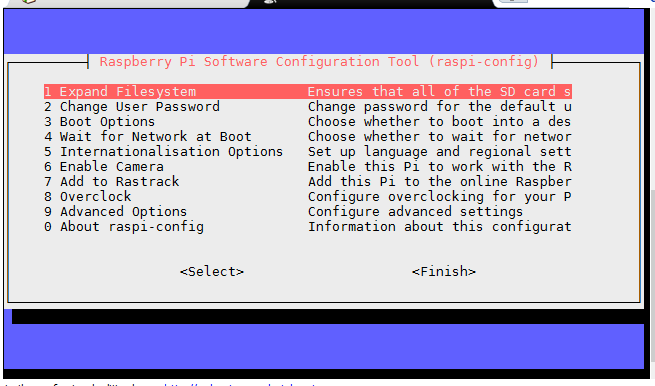
\includegraphics[width=11cm,height=5cm]{i2c_1.png}
			\centering
			\caption{[4]}
			\end{figure}
		\item Select the \textit{Advanced options}
		\begin{figure}[h!]
			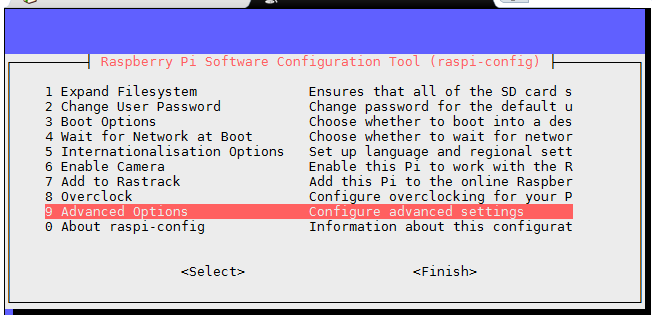
\includegraphics[scale=0.6]{i2c_2.png}
			\centering
			\caption{[4]}
		\end{figure} 
		\item Then select \textit{option A7 I2C} 
		\newline
		\begin{figure}[h!]
			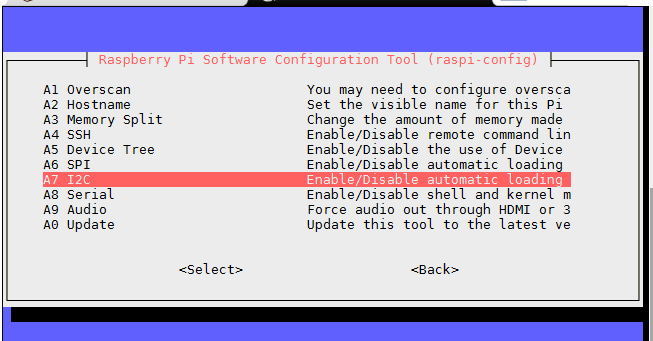
\includegraphics[scale=0.6]{i2c_3.png}
			\centering
			\caption{[4]}
		\end{figure}
		\item It will ask to enable the ARM I2C interface, click \textit{YES}.
		\newline
		\begin{figure}[h!]
			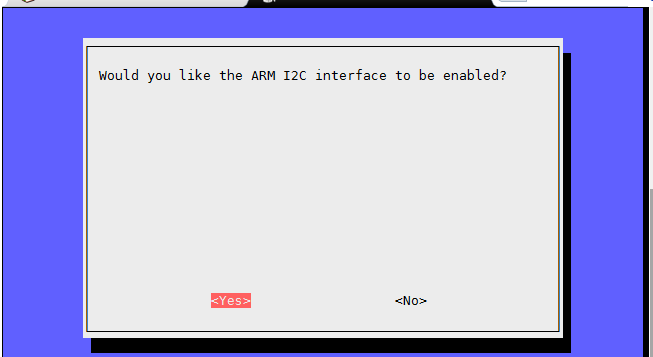
\includegraphics[scale=0.6]{i2c_4.png}
			\centering
			\caption{[4]}
		\end{figure}
		\newpage
		\item Then it will ask if you would like I2C kernel module to be uploaded by default. Select\textit{YES}.
		\begin{figure}[h!]
			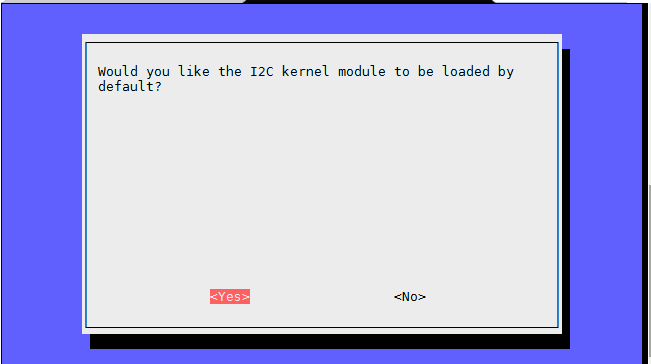
\includegraphics[scale=0.6]{i2c_5.png}
			\centering
			\caption{[4]}
		\end{figure}
		\item I2C kernel module will now be loaded by default.Click \textit{OK}
		\begin{figure}[h!]
			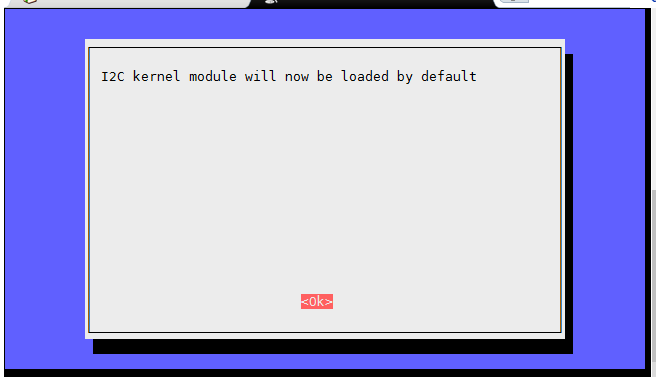
\includegraphics[scale=0.6]{i2c_6.png}
			\centering
			\caption{[4]}
		\end{figure}
		\item Select Finish to return to command line.
		\item Next we need to edit the modules file using : \newline \textit{sudo nano /etc/modules} 
		\begin{figure}[h!]
			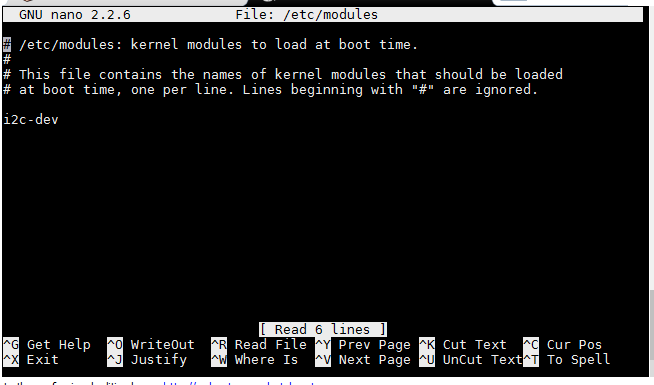
\includegraphics[scale=0.6]{i2c_7.png}
			\centering
			\caption{[4]}
		\end{figure}
		\newpage
		\item Add the following two lines : \newline \textit{i2c-bcm2708 \newline i2c-dev}
		
		\begin{figure}[h!]
			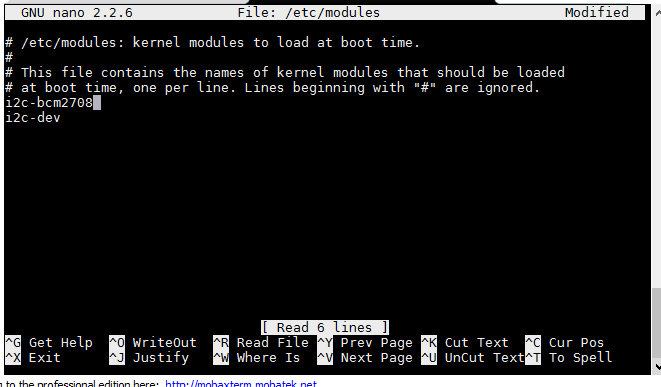
\includegraphics[scale=0.6]{i2c_8.png}
			\centering
			\caption{[4]}
		\end{figure}
		\item Use CTRL-X, then Y, then RETURN to save the file and exit.
		\item To help debugging and allow the i2c interface to be used within Python we can install “python-smbus” and “i2c-tools” : \newline \textit{sudo apt-get update \newline sudo apt-get install -y python-smbus i2c-tools}
		\item Shutdown your Pi using : \newline \textit{sudo halt} \newline Wait ten seconds, disconnect the power to your Pi and you are now ready to connect your I2C hardware.
		\item When you power up or reboot your Pi you can check the i2c module is running by using the following command : \newline \textit{lsmod | grep i2c\_} \newline That will list all the modules starting with “i2c\_”. If it lists “i2c\_bcm2708” then the module is running correctly.
		\item Once you have connected your hardware double check the wiring. Make sure 3.3V is going to the correct pins and you have got not short circuits. Power up the Pi and wait for it to boot.
		\item Type the command: \newline \textit{sudo i2cdetect -y 1} 
		\item You should the output as:
			\begin{figure}[h!]
				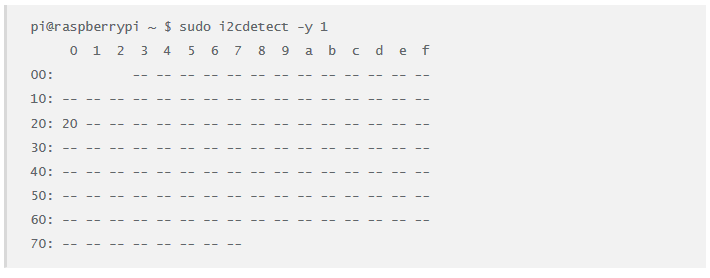
\includegraphics[scale=0.6]{i2c_9.png}
				\centering
				\caption{[4]}
			\end{figure}	
	\end{enumerate}
	
	\newpage

	\section{Appendix}
	\subsection{Raspberry Pi 2 Pin-out Diagram}
	\begin{figure}[h!]
		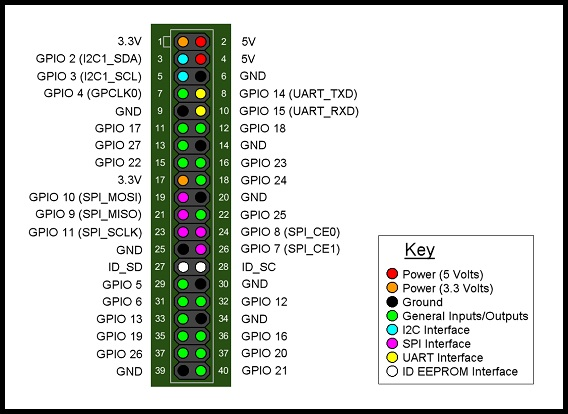
\includegraphics[scale=0.6]{RaspberryPi2_pinout.jpg}
		\centering
		\caption{[7]}
	\end{figure}
	
    \section{References}
    \begin{enumerate}
    	\item \url{http://www.byteparadigm.com/applications/introduction-to-i2c-and-spi-protocols/}
    	\item \url{https://learn.adafruit.com/adafruits-raspberry-pi-lesson-4-gpio-setup/configuring-i2c}
    	\item \url{https://camo.githubusercontent.com/c80be3d0c9e3146cd09e15b7ddf07dbb8b7d40b8/687474703a2f2f692e696d6775722e636f6d2f4575524e722e706e67}
    	\item \url{http://data.designspark.info/uploads/images/53bc258dc6c0425cb44870b50ab30621}
    \end{enumerate}
    
\end{document}



